% twocolumn を使うと2段組になる

%\documentclass[a4j,twocolumn]{jsarticle}        % -> platex
%\documentclass[a4j,twocolumn]{ujarticle}       % -> uplatex
\documentclass[uplatex]{jsarticle}   % -> uplatex + jsarticle

\usepackage{resume} % 他パッケージ,専用コマンド,余白の設定が書かれている

%%%%%%%%%%%%%%%%%%%%%%%%%%%%%%%%%%%%%%%%%%%%%%%%%%%%%%%%%%%%%%%%%%%%%%%%
% ヘッダ: イベント名,日付,所属,タイトル,氏名
%%%%%%%%%%%%%%%%%%%%%%%%%%%%%%%%%%%%%%%%%%%%%%%%%%%%%%%%%%%%%%%%%%%%%%%%

\pagestyle{plain}
\newcommand{\comment}[1]{}
\begin{document}
\twocolumn[
\beginheader{令和4年度 コンピュータサイエンス学部 中間発表}{2022}{8}{8}{井上 研究室}
\title{HMDを用いた怪獣体験ができるシミュレーションゲームの提案
}
\author{C0119127 斎藤 遥音 (Haruto Saito) }
\endheader
]

\vspace{3mm}

 % 本番用ページ番号オフセット
\setcounter{page}{1}

%---------------------------------------------------------------------------
% 本文
%---------------------------------------------------------------------------


\section{はじめに}
ゲームをするとき,現実では味わえないような経験ができる.その中でも人間以外のものになることができるゲームが多数ある。中でも怪獣に注目すると,カプコンから発表された特撮体感VR大怪獣カプドン~[1]というゲームでは、VR空間内で自由に街を歩き回ることができ,町を破壊することができる.しかし、一般的に怪獣は人間の何倍も大きさがあるため,HMDとコントローラのみで,簡単な装置をつけるだけだったため,怪獣特有の重量感や行動を体感することはできてなかった.

そこで,本研究では,プレイヤーの足がついた瞬間に足を振動させることで,重量感のある怪獣が歩いているような感覚を提示し,さらに火の息を吐くと,周りが燃え出したりすることで,より怪獣を体感することができるシミュレーションゲームを提案する.

\section{関連研究}
重量感を提示した研究として,河合らの研究~[2]では,重量感を提示する手法として,クロスモーダル効果を利用した.ダンベルを持ち上げる際のダンベルの移動距離を,VR空間内では短くしたり,持ち上げる際の時間を長くしたことで重量感を提示した.しかし,ダンベルを持ち上げる際に感じるダンベル自体の重さを感じることはできていないと判断した.

息検出を用いた研究~[3]として,檜山らの研究では,HMDに内蔵されているマイクを使用して,吹くことで吹き矢が飛び出す研究を行った.
この研究では,現実では何も持たずに行っていたため,息を吐く際の物理的な感覚としてのフィードバックが足りないという意見があったが,
本研究のように何も道具を用いる必要がない場合は,物理的なフィードバックは必要なくなるので,この手法が有効だと考えられる.

また,怪獣に着目した研究として,広田らの研究~[4]では,怪獣を生み出し実際に街の破壊などを行った.この研究ではHMDとコントローラにより頭部と両手のデータを取得し,足の動きについてはそれらのデータからIK(インバースキネマティクス)を使って行っており,実際の移動はコントローラのトラックパッドを使用している.
しかし,本研究では着足時の振動を重視したいため,現実の着足時同期させる必要があるため,コントローラでの移動では難しいと判断した.

\section{システム概要}
システム概要の図を図\ref{fig:system1}に示す.プレイヤーはHMDとコントローラに加え,足に加速度センサと振動モータを装着する.
また,VR環境を構築するソフトウェアとしてUnityを用いている.
怪獣視点になったプレイヤーはVR空間内を自由に歩き回ってもらい,コントローラを振ることで,周囲にある建物を破壊したりすることができる.
%もしかしたらケーブルの関係上自由に歩き回るのは無理かも
%できれば炎の息の後足元から温度を感じるようにしたい
%振動モータが無理なら床からのサブウーファー
そして歩く際に,着足するたびにプレイヤーに振動がいきわたる.
さらに、息を使って炎の息を吐いてもらう際,地面に炎の息が当たると,その部分が燃えるようになる.

\begin{figure}
 \begin{center}
    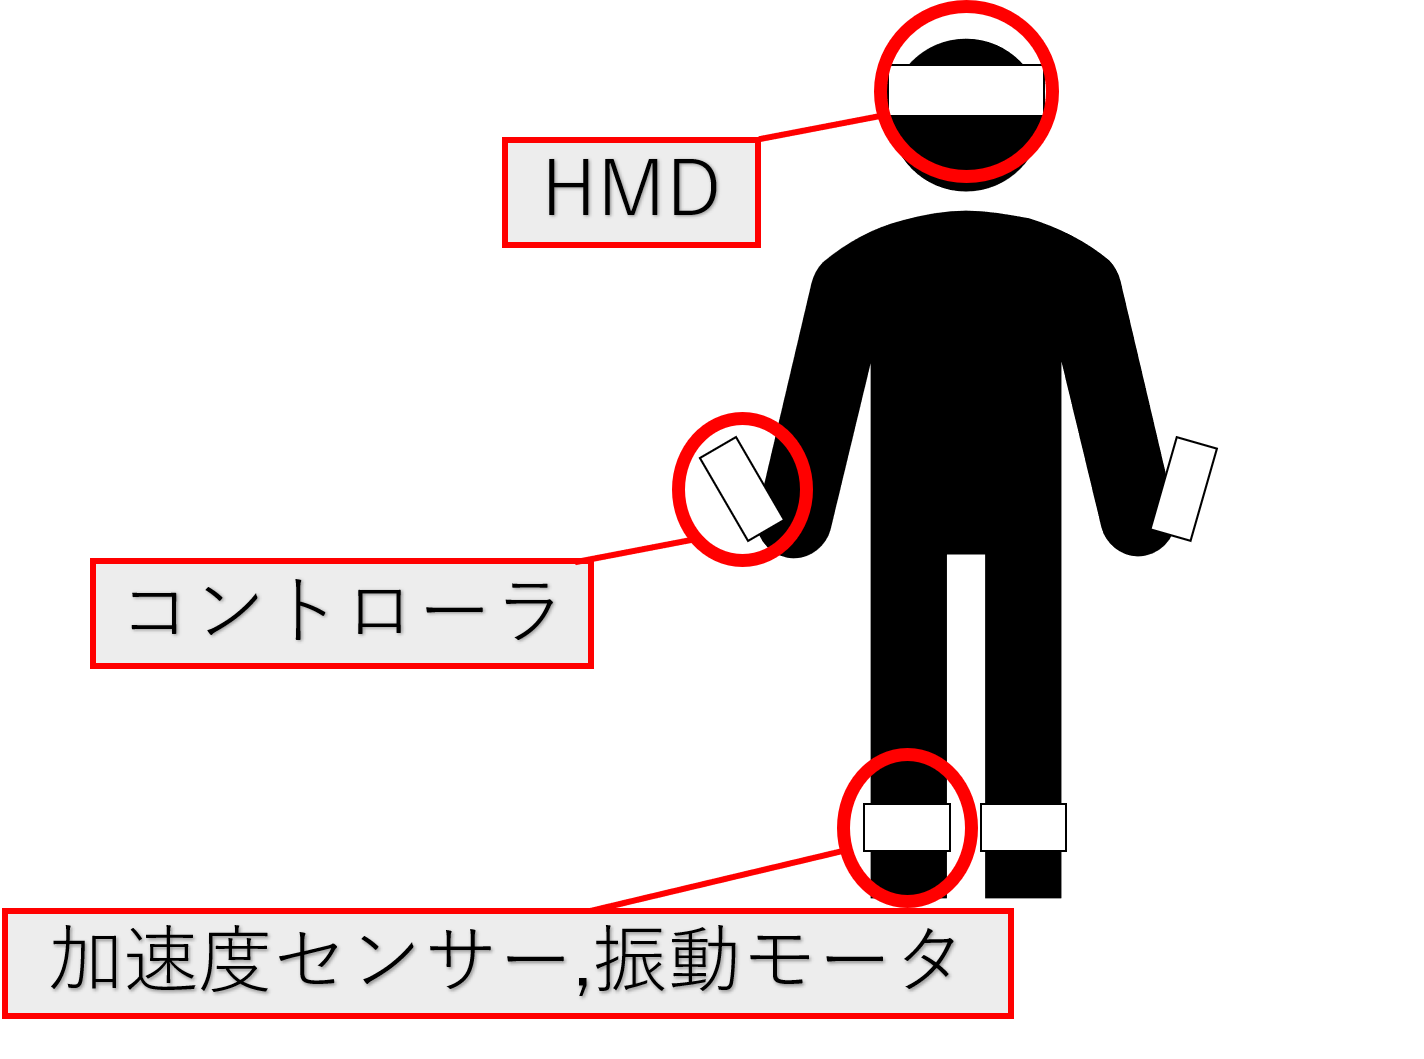
\includegraphics[width=0.75\linewidth]{fig/system1.png}
 \end{center}
    \caption{システム概要}
    \label{fig:system1}
\end{figure}

\section{システム構成}
システム概要の図を図\ref{fig:system2}に示す.
HMDやコントローラや加速度センサから得られるデータをPCに送る.
送られたデータをもとに怪獣の視点を自由に動かしたり自由に歩き回ることができる.
また加速度センサの情報をもとに歩行認識を行い,VR空間内で足の上げ下げをおこなう.着足時には,足の振動を行うために,足に取り付けた振動モータを振動させている.
そして,息の検出については,HMDに内蔵されているマイクを使用しており,プレイヤーが息を吹きかけ,それをマイクが認識すると,炎の息がでるようになっている.

\begin{figure}
 \begin{center}
    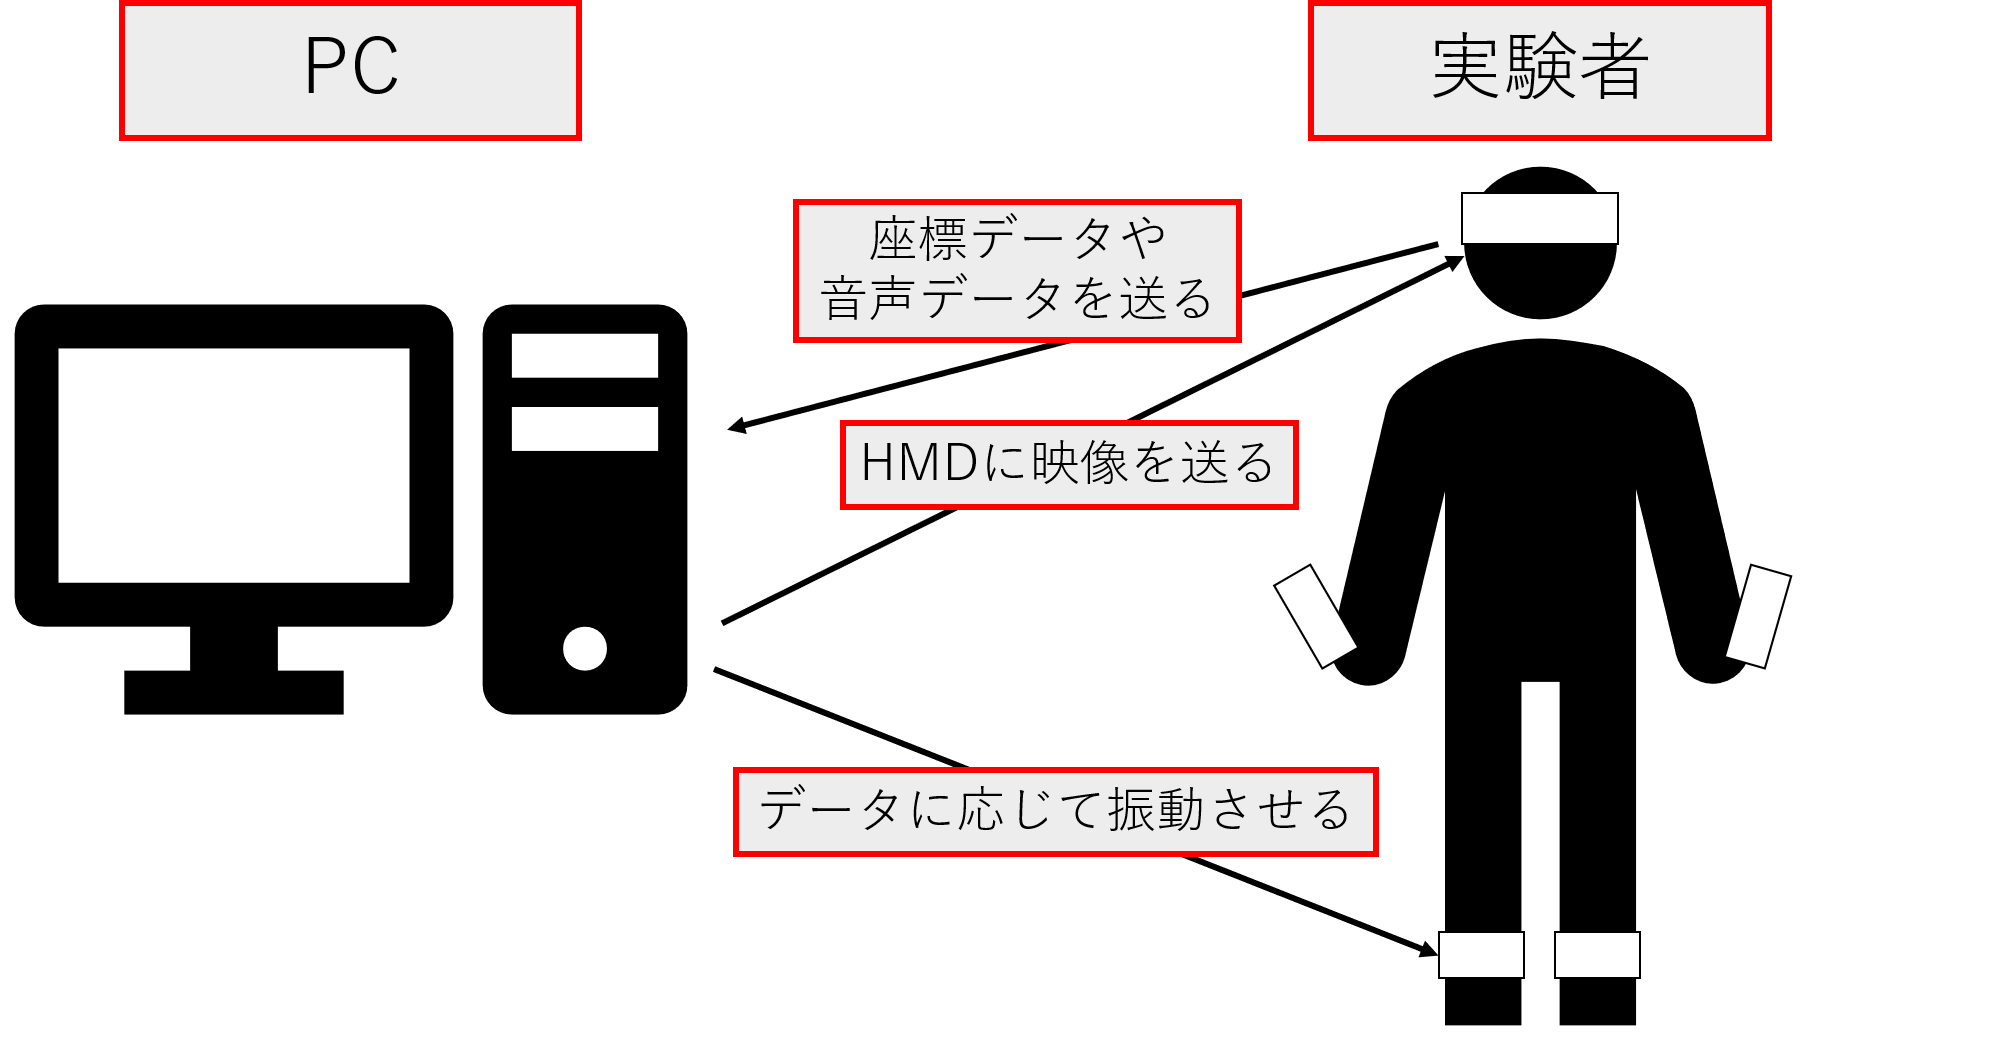
\includegraphics[width=0.75\linewidth]{fig/system2.png}
 \end{center}
    \caption{システム構成}
    \label{fig:system2}
\end{figure}

\section{実験方法}
\subsection{実験手順}
本実験では2種類の実験を行う.
実験参加者はHMDとコントローラと加速度センサーと振動モータを装着してもらう.
最初に自由に歩き回ってもらい特に問題がなかったら実験を開始する.
実験1では,関連研究~[1]のように,自由な移動と手での破壊行為のみで行ってもらう.
周囲にあるビルなどの建物をすべて破壊することができたら,実験終了とする.

実験2では実験1に加え床からの振動と炎の息の要素を加えて,同様に自由に動き回ってもらう.
こちらも同様に周囲にあるビルなどの建物をすべて破壊することができたら,実験終了とする.

また、それぞれの実験ごとにアンケートを実施する.

\subsection{アンケート方法}
このアンケートによって,実験参加者が怪獣を体感できたかを行う.また既存の手法と比べてどのような点で怪獣を体感できたか調査を行う.
アンケートは5段階評価で答えてもらう.
実験1の後で答えてもらうアンケートでは,全体を通じて怪獣を体感できたか,歩いて街を破壊する行為に違和感はなかったか,手で街を破壊する行為に違和感はなかったかなどの質問に答えてもらう.
実験2の後で答えてもらうアンケートでは,先ほどの質問内容に加えて,炎の息によって燃やす行為に違和感はなかったかなどの質問に答えてもらう.
その後2つのアンケート内容をもとに比較を行う.実験2の結果のほうが高い評価を得られた場合は,提案手法に優位性があったということになる.

\section{検討事項}
本論文では主な検討事項が2つある.

一つ目は炎の息を吐く際にマイクを使用しているため,息以外にも話したりするだけでも炎の息を吐いてしまう点である.
そのため,息だけ反応するような装置を検討する必要がある.

二つ目は町の建物が当たった際に生じる衝撃の点である.ビルなどの高さによって,足以外にも手や胴体部分にもあたる可能性があるため,当たった部分が振動するように検討する必要がある.

\section{まとめ}
本論文ではより怪獣を体験をするため,足の振動や炎の息を加えた怪獣体験のシミュレーションゲームを提案した.今後はさらに行動を増やし,さらなるクオリティアップを検討する.

%---------------------------------------------------------------------------
% 本文終わり
%---------------------------------------------------------------------------

 % 参考文献

\begin{thebibliography}{99}
    \item カプコン,特撮体感VR 大怪獣カプドン,2017,https://www.capcom.co.jp/arcade/capdom/,(2022-08-01)
    
    \item 平尾 悠太朗,三家 礼子,河合 隆史,VR空間におけるクロスモーダルを用いた重さ感覚提示手法の提案と評価,日本バーチャルリアリティ学会論文誌,2018,vol.23,No.4,pp.263-270
    
    \item 山野 孝太,佐々木 智也,宮崎 敦子,登嶋 健太,檜山 敦,VR吹き矢:呼気検出を用いた呼吸リハビリテーション,「エンタテインメントコンピューティングシンポジウム,2021
    
    \item 桜井 翔,武井 友里恵,野嶋 琢也,広田 光一,怪獣アバタを用いたバーチャル破壊体験による非主張性軽減手法の検討,第25回日本バーチャルリアリティ学会大会論文集,2020
    
\end{thebibliography}

\end{document}


%-----------------------------------------------------
% テンプレート
%------------------------------------------------------------------------------

%-----------
%% 箇条書き
%-----------
%\begin{itemize}
% \item
%\end{itemize}

%-------------------
%% 番号付き箇条書き
%-------------------
%\begin{enumerate}
% \item
%\end{enumerate}

%-----------
%% 図の表示
%-----------
%\begin{figure}[H]
% \centering
% \includegraphics[clip,width=7cm]{hoge.eps}
% \caption{図タイトル}\label{fig:hoge}
%\end{figure}

%-----------
%% 図の参照
%-----------
%\figref{fig:hoge}

%-----------
%% 表の作成
%-----------
%\begin{table}[H]
% \centering
% \caption{表タイトル}\label{tab:fuga}
% \begin{tabular}{|c|c|c|}\hline
%  hemo & piyo & fuga \\ \hline
%  hemo & piyo & fuga \\ \hline
% \end{tabular}
%\end{table}

%-----------
%% 表の参照
%-----------
%\tabref{tab:fuga}

%-----------
%% 参考文献
%-----------
%\begin{thebibliography}{9}
% \bibitem{piyo} 参考文献
%\end{thebibliography}

%-----------------
%% 参考文献の参照
%-----------------
%\cite{piyo}
